\documentclass[12pt]{article}
\usepackage{graphicx}
\usepackage[margin=1in]{geometry}
\usepackage{url}

\begin{document}
\begin{figure}
	\begin{center} 
\includegraphics[width=0.2\linewidth]{maklogo.png} \end{center}
\end{figure}

	\begin{center} \begin{Large} \textbf { COLLEGE OF COMPUTING  AND INFORMATION SCIENCES} \end{Large}  \end{center} 
	\begin{center} \begin{Large} A programming assignment autograder for moodle \end{Large} \end{center}
	\begin{center} \begin{Large} By \end{Large} \end{center}
	\begin{center} \begin{Large} CS18-02\\[1in] \end{Large} \end{center}
	
	\begin{center} \begin{Large} \textbf {DEPARTMENT OF COMPUTER SCIENCE} \end{Large}  \end{center}
	\begin{center} \begin{Large} \textbf {SCHOOL OF COMPUTING AND INFORMATICS TECHNOLOGY\\[1in]} \end{Large}  \end{center}
	\begin{center}A Project Proposal Submitted to the School of Computing and Informatics Technology
For the Study Leading to a Project Report in Partial Fulfillment of the
Requirements for the Award of the Degree of Bachelor of Science in Computer Science
Of Makerere University  \end{center}
\begin{center} \begin{large} \textbf { Supervisor} \end{large}  \end{center}
\begin{center} \begin{large} Ernest Mwebaze \end{large}  \end{center}	
\begin{center} \begin{large} School of Computing and Informatics Technology, Makerere University \end{large}  \end{center}
\begin{center} \begin{large} emwebaze@gmail.com, +256-772-121-272 \end{large}  \end{center}
\begin{center} \begin{large}October, 2017 \end{large}  \end{center}
\newpage
\begin{center}\begin{Large}GROUP MEMBERSHIP \end{Large} \end{center}

\begin{tabular} {|c|c|c|c|}
\hline
SNo & Names & Registration  Number & Signature \\ \hline
1 & ABULE AUGUSTINE ARUMADRI &  15/U/2633/PS &  \\ \hline
2 & AYIKO JEREMIAH SARA &  15/U/186 & \\ \hline
3 & OWOMUGISHA ISAAC &  15/U/12351/PS & \\ \hline
3 & SENDIKADDIWA MARVIN &  15/U/1154 & \\ \hline
\end{tabular}
\newpage
\tableofcontents
\newpage
\section{Introduction}
	\subsection{Background}
		E-learning is a style of teaching and learning done over a network. It is independent of location and time constraints in regard to attendance. As soon as the materials (lectures notes, assignments, etc.) are uploaded, a student can access them at any time. It offers a way to design courses in a more interactive way e.g. through the use multimedia and is
		cost effective. Today, multiple universities all over the world use e-learning platforms to enhance understanding of course content such as Harvard, Stanford, and MIT \cite{singh}. With time more efficiently spent, multiple assignments can be given and automatically graded to identify and improve areas that the students did not understand fully. \\
		
		Moodle is an e-learning platform designed for educators, administrators and learners with a single robust, secure and integrated system to create personalized learning environments \cite{moodle}. It is easy to use and open source. Moodle will be used as the core system on which the e-learning platform will be designed. Makerere University already uses Moodle to run it's e-learning platform called MUELE \cite{muele}. We are building the system on top of moodle because of the overwhelming challenges involved in building a system from scratch (such as security considerations and user management issues).
	\subsection{Problem Statement}
		Monitoring each student's performance in Makerere university's classes is a tiresome task for lecturers. When students are given a programming course work, they expect fair and continuous feedback from their lecturers in the least time possible. However, at times students are given complex tasks to do as course work. For a lecturer to give reasonable feedback to every student's course work, he would be required to run the student’s code into the IDE to correctly analyze the running time, correctness and generate relevant feedback. Besides analyzing code efficiency and correctness of the code, the lecturer is also subjected to the task of checking for plagiarism among the submitted code. The current prevailing solution to improve the lecturer's productivity is grouping students. The problem with this is that only a few students contribute to the course work and the rest do not benefit. This is also not a permanent solution
		since only group effort is monitored at the expense of individual effort.
		
		This project's intention is to solve the above problem by creating an on-line system that will keep track of a student's individual progress in the programming field and monitoring the student's general performance in the least time possible. With this implemented, student's submitted course work will be attended to quickly, plagiarism acts will be detected, teachers' productivity will be improved and student's passion for programming and computer science will be boosted.
	\subsection{Objectives}
		\subsubsection{Main Objective}
		The general intention of the project is to develop a Moodle plugin that will automatically grade programming assignments uploaded to the system by students, keep track of each student’s performance based on scores attained from previously uploaded assignments and provide relevant feedback both to the students and the lecturer. The system should also enable lecturers to give in-class assignments for real-time assessment.
		\subsubsection{Specific Objectives}
		\begin{itemize}
			\item To design a Moodle plugin that will automatically grade the submitted programming assignments.
			\item To do literature review on existing E-learning systems. 
			\item To implement the proposed system.
			\item To test the system to ensure that it meets the specified requirements.
		\end{itemize}
		
	\subsection{Scope}
		Computer programs and source code exist in many programming languages and size (in terms of actual lines of code) and they require different computer resource to execute properly. In order to support a broad range of courses, it is important to build a general platform that can support as many languages as possible. However, the aim of this project is to build a proof of concept platform. Thus, we mainly be concentrating on the C and Java programming languages.
		However, in the future we want the system to be platform independent. \\
		 
		When designing a platform used for automatic grading purposes, accurate assessment is of utmost importance. The programming assignments must therefore be tailored with the intention of keep the auto-grading process simple and and stable while at the same time challenging and relevant to students in order to hone their programming skills at the same time pass that particular course unit. Another important aspect is user feedback. The system is designed to be a substitute of the lecturer when it comes to assessment. Therefore it must provide relevant feedback to the students regarding use of better or correct algorithms, and also to the lecturer on topics where students are finding challenges.\\
		
		For purposes of testing the effectiveness of the working system, we will focus on
		programming course units taught in the Computer Science course only within Makerere
		University. Programming languages covered in this course are C and Java.

	\subsection{Significance}
			A delivered working system will be of great help to both students and lecturers who use it
		as part of their teaching tools. Many at times students do not get the personal attention
		from lecturers as they so do desire. This may be attributed to the large number of students
		offering a particular course unit, each most likely with their unique challenges they face.
		There also exists the general perception that university students are not supposed to be
		spoon-fed, but rather engage in rigorous research and extensive personal reading. Much
		as this encourages academic independence, many students need one on one academic
		guidance. Our auto grading system provides this guidance. \\ \\
			By having the ability to suggest better algorithms and language structures/functions to use,
		each student can be guided on better coding techniques and how to optimize their programs. In the current setup at 				CIT, this is very difficult to achieve through manual means by the lecturer. \\ \\
			By enabling the lecturer to give in-class assignments that can be automatically graded,
		students are encouraged to constantly practice programming skills in order to be prepared
		for these assignments. This has a direct positive impact on their academic performance in
		that particular course unit, at the same time improving their general programming skills
		even though not examinable. 

\newpage

\section{Literature Review}
	In this section, we provide a summary the previous work that has been done on E-learning platforms, auto-graders and online judges.
	
	Many of the leading universities of computer science education around the world incorporate auto grading in their 			programming and algorithms courses. For example, in 2013, MIT researchers Singh et al \cite{singh} introduced a new method for automatically providing feedback for introductory programming problems. According to \cite{ojpot}, due to fair and timely feedback results from online judge websites, online practice outperforms traditional programming practice.

	\subsection{Related work}
		\subsubsection{MUELE and Moodle}
		MUELE (Makerere University E-learning Environment) \cite{muele} is the dominant e-learning platform used at Makerere University. It is used for publishing notes and assignments for students. It also has functionality for giving on-line quizzes (mainly objective type and single-response questions). MUELE is based on the moodle online learning platform.
		
		One of the most dominant e-learning platform used worldwide is Moodle. The moodle website \cite{moodle} states that ``Moodle is a free and open-source software 	learning management system written in PHP and distributed under the GNU General Public License. Developed on pedagogical principles, Moodle is used for blended learning, distance education, flipped classroom and other e-learning projects in schools, universities, workplaces and other sectors." The Moodle platform is composed of several “components” that enable its dynamism and thus can be adopted for the project.
		
		``Plugins are a flexible tool set, allowing Moodle users to extend the features of the site" \cite{moodle}. Plugins for moodle can be thought of as modules or widgets with specific functionality. Currently moodle is consists of thousands of plugins developed to suite different teaching curriculum. Some of the existing plugins relevant to our project are: URKUND plagiarism plugin \cite{urkund} used for checking plagiarism in submitted files and Reengagement plugin \cite{reengagement} for sending timely feedbacks to remind students of uncompleted course activities. Since some of these plugins are open source, they can be used as sub modules in our project.
		\subsubsection{Building plugins for Moodle}
		Moodle has a well-structured documentation to help developers write plugins from start to publishing them on the 			website for usage. The prerequisites for plugin development are: -
		\begin{itemize}
			\item  Comfort using (Hypertext preprocessor file) PHP.
			\item  Ability to install a database and a web server on a local machine.
		\end{itemize}
		 Resources for programmers with no skills of prerequisites are provided in the documentation. These include PHP 				tutorials for novice programmers and database installation video tutorials links to YouTube.
		 If you download Moodle source code or clone it from git, you will see a bunch of files and folders. This code 				consists of Moodle core (that consists of the Very core and Core components), third party libraries and plugins.  			Moodle has 24 different categories of plugins\cite{moodle} and uses git for development. If one wishes to develop a plugin and 			finds out it has already been developed, then they may opt to contribute to its code. For one to develop a new kind 		of plugin, a skeleton of a plugin is provided (template) with basic PHP code that displays a simple page. This only 				contains the “page” API which all plugins that display something on the webpage include. The documentation 				continues to explain the cloned repository file structure, callbacks, Core APIs, adding basic contents to your page, 			to publishing your plugin into Moodle’s Navigation. A further documented tutorial to manipulate Databases in Moodle 		is provided for advanced plugins development.
		 \subsubsection{Plugins for Moodle}
		 Moodle has thousands of plugins each falling in different categories/types. Some of these are :- 
		 \begin{itemize}
			\item Anti-viruses: which check for viruses in uploaded submitted files. “Antivirus scanner plugins provide 						functionality for virus scanning user uploaded files using third-party virus scanning tools in Moodle. For 				example: ClamAV.” 
			\item  Quiz reports: For displaying and analyzing the results of quizzes, or just plug miscellaneous behavior 					into the quiz module.
			\item Question types: Different types of question (e.g. multiple-choice, drag-and-drop) that can be used in 					quizzes and other activities.
			\item Question behaviors: Control how student interact with questions during an attempt.
			\item Plagiarism plugins: Define external services to process submitted files and content. The files handled 						include reports and programming work.
		\end{itemize}
		As far as programming assignment plugins are concerned, the only plugin developed is “Programming Code 				Plagiarism”. “This plugin integrates two well-known source code plagiarism detectors MOSS and JPlag into Moodle to 			compare the similarities of programming assignments of students within the same course. By integrating these 				detectors seamlessly into Moodle, it eliminates the overhead of manually preparing the assignments to feed into 				these detectors, present the reports with an interactive interface and, more importantly, serve as an educational 			tool to provide feedback to students and raise their awareness of plagiarism.” The plugin has a comparison view 			that looks for similarities in work done by one student to the rest of the students. By ticking the checkbox "Show 				similarity between someone with other students", lecturers can also see the similar parts of that students with 			everyone in the class (not just pair to pair).
		 \subsubsection{Auto-graders/Assessment plugins for Moodle}
		 On Moodle, a lecturer/instructor can add an assignment activity for students. This involves describing the 					assignment nature where a series of steps are attended to in a chronological order viz. Assignment name, 					description, Due date, require students to click submit button, etc. As far as our project is concerned, the most 				interesting part on the assignment settings is Grading. There are three options to choose a grading method. Viz. 				simple direct grading (entering a grade or scale item), Marking guide and Rubric. \\
		 \textbf{Marking guide}: A marking guide is an advanced grading method where a teacher enters a comment per 				criterion and a mark up to a maximum. This involves creating a marking guide that is to be followed by students and 			markers in order to know what is required and the maximum mark per criterion is provided too. This process involves 		creating a set of criterions and to avoid duplicates, criterions can be added to “frequently used criterions” section. 			This is a manual marking guide that the teacher will follow after students submit their solutions. \\
		 \textbf{Rubric}: “Rubrics are advanced grading forms used for criteria-based assessment. The rubric consists of a 			set of criteria. For each criterion, several descriptive levels are provided. A numerical grade is assigned to each of 			these levels. The rater chooses which level answers/describes the given criterion best. The raw rubric score is 				calculated as a sum of all criteria grades. The final grade is calculated by comparing the actual score with the worst/			best possible score that could be received.”
		\subsubsection{Online judges and autograders}
		The most popular application of online judges is in programming contests such as TopCoder, ACM/ICPC and Google Code Jam. The most prominent of these is the ACM/ICPC \cite{icpc}. The ACM/ICPC consists of algorithmic and programming problems for contestants to solve. The contestants' submissions are evaluated based on the output of their programs. A typical problem in this contest consists of the following parts:
		\begin{itemize}
			\item Problem description: This is a description of the problem to be solved.
			\item  Input description: This gives the specification of the input file from which the user’s
				solution programs read data
			\item Output description: This specifies the format in which the program should produce
				results.
			\item Sample input and sample output: These provide examples to clarify the input and output
				specifications.
		\end{itemize}

		For each problem in ACM/ICPC, there are multiple sets of data to be processed. This is an important feature that serves two major purposes \cite{ojpot}: first, they are used to test that the program can work in all possible situations (including corner cases). Second, they are used to calculate the running time of a program (a good solution should be able to work on both small datasets and larger datasets). The use of multiple datasets therefore ensures that a student’s submission is evaluated comprehensively. 
		
		Test datasets of problems in the ACM/ICPC are either generated by hand for small-sized datasets or by programs written by jury members that generate datasets according to some predefined patterns or at random \cite{budzalov}.
		
		In \cite{anti}, Dr. Antti Laaksonen describes how a competitive programming approach using an online judge to teach algorithm concepts has helped improve the problem solving skills of the students at the University of Helsinki. In 		the course, the TMC system \cite{tmc} is used. TMC allows students to create their Java solutions in the NetBeans IDE and evaluates the solutions using JUnit tests. The tests are written by the course staff. In this paper, he describes how this model of teaching helps students understand the importance of developing efficient algorithms. He also points out some limitations of using online judges. He gives an example of the following problem from \cite{clrs}:
		
		Describe an $O(n)$-time algorithm that, given a set $S$ of $𝑛$ distinct numbers and a positive integer $k \leq n$, determines the $k$ numbers in $S$ that are closest to the median of $S$. 
		
		He points out the difficulty of automatically determining whether a student’s submission of the above problem is really $O(n)$, since the same problem can be solved in $O(n log n)$ time. This therefore means that auto-graders are not perfect, however they seem to be better than traditional means of evaluation as the following section shows.

	\subsection{Benefits of auto-grading and practice oriented teaching of programming}
		Researchers Wang GP et al. conducted two sets of experiments \cite{ojpot} in order to evaluate the effectiveness and validity of using their online judge system called OJPOT as compared to traditional teaching methods. They set out to answer the following questions \cite{ojpot}:
		\begin{itemize}
			\item  Does OJPOT work effectively to enhance students' practical abilities compared to the
					traditional teaching idea?
			\item  In which aspects can OJPOT improve the student's practical abilities?
			\item Output description: This specifies the format in which the program should produce results.
		\end{itemize}
		In the first set of experiments, two classes were chosen: one class defined as the control class (CC) and another defined as the experimental class (EC). In the CC, the traditional teaching idea was applied; while in the EC, the OJPOT online judge was used \cite{ojpot}. Before the experiment, both classes were given a pre-test to evaluate their elementary knowledge in C programming. Then during the semester, both classes were taught by the same teacher with the same timetable. The following data were collected during the experiment: pre-test scores, online practice and statistical data, post-test scores and course project scores. Below is a summary of the results of their experiment (\cite{ojpot}):
		\begin{itemize}
			\item Both classes had similar programming foundation before the experiment
			\item At the end of the semester, there were significant differences between the CC class and
				the EC class: the EC class has overall better results in the final tests and project.
		\end{itemize}
		They conclude their results by remarking that the EC class performed better because the online
	judge system made the students more enthusiastic about the material they were studying. It was
	also observed that the general programming abilities of the EC class were improved much better
	than those of the control class. 
	
	\subsection{Conclusion}
	In computing, time is an important aspect. This can be taken care of if we avoid creating already existing technology 			“reinventing the wheel”. If we are to create our own project from scratch it will be tedious. We will be required to design a 		whole complete site with a perfect interface and backend functionality for the project to be viable. With the presence of 		existing open source projects like the one cited above i.e. Moodle, we can collaborate with them and contribute to their 			source code. In so doing, the advantages encountered will be:- 
	 \begin{itemize}
			\item More time to concentrate on the project’s main functionality and objectives.
			\item 	After development, the project will not be rendered trivial. Moodle being a popular platform 							worldwide, our efforts of marketing for a system would be exponentially reduced to zero.
			\item	The main institute we are targeting to use our project’s deliverable (plugin) is Makerere University. As 					stated earlier, this institute has its own E-Learning Environment (MUELE) which also runs on the 						Moodle framework. Thus, implying that it can perfectly run any plugin run by the Moodle website.
		\end{itemize}

\newpage

\section{Methodology}
	In this section, we explain the methods and tools that we're going to use to complete this project. The proposed system is going to be built as a plugin for the Moodle online learning platform. It will consist of a website and a mobile application. Users of the system will be lecturers and students.
	\subsection{Implementing the Auto-grader/on-line judge}
		\subsubsection{Method of grading}
		Grading shall be done by comparing the result of a student's submissions to the expected result. The students are going to be submitting their programs through a web interface, these programs shall be ran in the back-end and tested on various test data to determine the correctness of the student's solution. 
		
		Besides correct output, the lecturer might want the students' submissions to meet other requirements such as API specification, coding style or use of a particular language feature. In order to check that these requirements are met, the system shall use tools such as checkstyle \cite{checkstyle} and PMD \cite{pmd}. These tools provide mechanisms for extensive source code analysis.
		\subsubsection{Limiting resources}
		Since computer resources are finite, we have to incorporate a mechanism that limits how much resources the students' submission uses. Some of the resources to be limited include time, memory usage and access to restricted features of a language (for example features that could lead to security breaches). This can be done by running the code inside a virtual machine such that malicious code cannot affect the servers and the overall system. To limit amount of time used, a script that keeps track of how long the code has been running will be used to terminate the execution and send a “Time Limit Exceeded” verdict to the student if their code takes too long to run. A similar approach will be used to enforce memory usage constraints.
		\subsubsection{Tools available for the lecturer}
		The proposed system shall include a simple tool to allow lecturers to prepare assignments. This tool will enable lecturers to create model solutions to the assignments whose output will be compared to the student’s output. The tool will also provide an API to enable the lecturers to generate test data.
	\subsection{Implementing Analytics and other evaluation metrics}
	Various kinds of data will be collected from users' interaction with the system. This data includes (but is not limited to): number of tries a student uses to get the correct solution, number of students that have successfully completed a particular assignment, average score of students and difference in scores for assignments in particular topics.
	
	We intend to use this data that is collected to provide useful feedback to lecturers in order for them to gauge how well they are teaching a particular course unit and where they can make improvements. Students shall also get feedback that will enable them to see where their weaknesses are and help	them improve. We are going to explore various machine-learning algorithms in order to see how best to make use of this data. An example use of the data is determining the difficulty of a problem (or assignment) and the skills of a student. Given that we have collected data about how long it takes various students solve a problem, we can formulate this as a machine learning/statistics problem of the following form:
	\begin{itemize}
		\item Data is of the form: Student $s$ solved problem $p$ in time $t_{sp}$.
		\item We need to estimate student skills and problem parameters used for determining how difficult a problem is. 
	\end{itemize}
	With a proper formulation of the problem, we can then apply algorithms such as gradient-descent \cite{gds} or a collaborative filtering algorithm like “SVD” \cite{kalman} to make recommendations and provide insights into individual and general performance of the class.
	\subsection{Implementing on top of Moodle}
	Moodle\cite{moodle} is an open source platform for educators to develop and manage courses online. It's a modular system based on plugins. We plan on building this system as a plugin for Moodle. Moodle uses PHP as its underlying programming language and thus the components of this project will be primarily written in PHP. Building our proposed system on top of Moodle will ensure that we do not have to worry about issues like user management and security thus enabling us to focus on the core functionality of the application.
	\subsection{Testing the system}
	We plan on testing the system in a real classroom environment. Once the system is functional, we shall request a lecturer who teaches a programming related course unit to try out the system in his class. In the testing phase, we shall seek to answer the following questions:
	\begin{itemize}
		\item Does the system meet the functional and non-functional requirements (which are highlighted in the software requirements specification document)?
		\item Can the system be used without issues for giving assignments? This is to determine the system reliability and usability. (This will be determined by monitoring logs for crashes and other issues that may arise).
		\item Does the system improve on how programming assignments are given in Makerere University as compared to current methods? (This shall be determined by giving surveys to the students and the lecturers.)
	\end{itemize}
	
	In addition, we shall write comprehensive unit-tests to ensure that the system has expected behavior.

\newpage
\bibliography{references}
\bibliographystyle{ieeetr}
\newpage
\section{Appendices}
\subsection{Appendix A: Activities Gantt chart}
\begin{figure}[h]
	\begin{center} 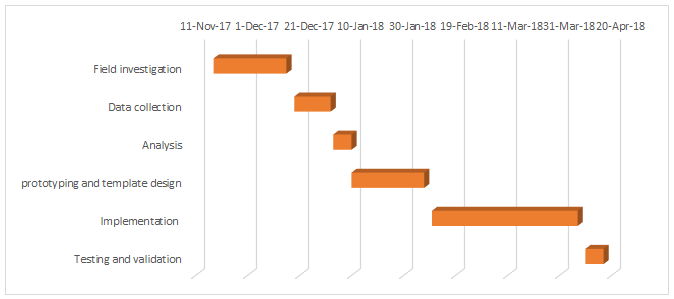
\includegraphics[width=1\linewidth]{gantt.png} \end{center}
\end{figure}
\subsection{Appendix B: Financial Requirements}
\begin{tabular} {|c|c|c|c|}
	\hline
	Requirement & Quantity & Unit price (UShs) & Total price \\ \hline
	Generating questionnaires & 50 &  1,000 & 50,000 \\ \hline
	Data(Internet) & 20gb &  12,000 & 240,000 \\ \hline
	Private GitHub repository & 1 &  32,400(per month) & 64, 800\\ \hline
	Miscellaneous & -  & 100,000 & 100,000\\ \hline
	Total &  &  & 454,800\\ \hline
\end{tabular}
\end{document}